\header{
    \section{Auprès de ma blonde} \label{aupres-de-ma-blonde}
    %
    
    \insertComment{Complainte d'une hollandaise au mari prisonnier lors de la guerre de Hollande (1672-1678) publiée en 1704 sous le titre "Le prisonnier de Hollande".}{}
    %Fun fact : Elvis Presley l'a chantée en 1967 dans le film Double Trouble.
    %Version de Presley : https://www.youtube.com/watch?v=ito_RR2kwS0

    \vspace{-0.5cm}
}

\enluminure{4}{\href{https://www.youtube.com/watch?v=AjEIVO9Xitk}{D}}\\ 
$\left.\begin{tabular}{l}
\hspace{-0.4cm}
\textsc{ans} les jardins d'mon père 
\\
\hspace{-0.4cm}
Les lilas sont fleuris
\end{tabular}\right\rbrace$ bis
\\Tous les oiseaux du monde 
\\Viennent y faire leur nid.
\\\\\textbf{Refrain :}
\\Auprès de ma blonde 
\\Qu'il fait bon, fait bon, fait bon 
\\Auprès de ma blonde 
\\Qu'il fait bon dormir.
\\
\bisdouble{La caill', la tourterelle  ~~~~~~}
{Et la jolie perdrix.}
\\Et la jolie  colombe 
\\Qui chante jour et nuit. 
\\
\bisdouble{Qui chante pour les filles ~ }
{Qui n'ont pas de maris.}
\\Pour moi ne chante guère 
\\Car j'en ai un joli. 
\\
\bisdouble{Dites nous donc ma belle   ~~}
{Où est votre mari ?}
\\Il est dans la Hollande, 
\\Les hollandais l'ont pris. 
\\
\bisdouble{Que donn’riez-vous la belle }
{Pour avoir votre ami ?}
\\Je donnerais Versailles,  
\\Paris et Saint Denis. 
\\
\bisdouble{Les tours de Notre-Dame,  ~~~~~}
{Et l'clocher d'mon pays.}
\\Et la jolie colombe,
\\Pour chanter avec lui.
\\
%\bigskip
%\begin{figure}[h!]
%\centering
%   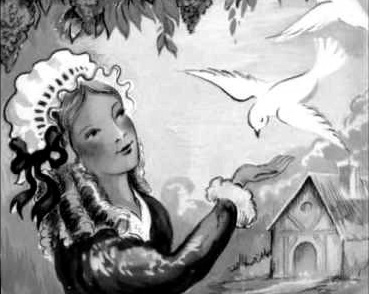
\includegraphics[width=0.9\textwidth]{images/blonde.jpg}
% \end{figure}

\breakpage


